\documentclass[bibtotoc,UKenglish,halfparskip,oneside,DIV12]{scrreprt}
\usepackage[latin1]{inputenc}
\usepackage[T1]{fontenc}
\usepackage{babel}
\usepackage{cmbright}
\usepackage{graphicx}
\usepackage{varioref}
\usepackage{xcolor}
\usepackage{pifont}

\definecolor{susepflaume}{rgb}{0,0,0.45}
\definecolor{listinggray}{gray}{0.95}

\usepackage{listings}
\lstset{%
        backgroundcolor=\color{listinggray},
        rulecolor=\color{listinggray},
        fillcolor=\color{listinggray},
        basicstyle=\ttfamily\small,%
        escapechar={},
        captionpos=b,
        columns=fullflexible,
        tabsize=4,
        showstringspaces=false,
        keepspaces=true,
        frame=tb,
        xleftmargin=8mm,
        xrightmargin=0mm,
        framexleftmargin=8mm,
        framextopmargin=1mm,
        framexbottommargin=1mm,
        numbers=left,
        numberstyle=\tiny\sffamily,
        stepnumber=1,
        firstnumber=1,
        aboveskip=\bigskipamount,
        belowskip=\bigskipamount
}
\lstdefinestyle{inline}{%
        frame=none,
        numbers=none,
        xleftmargin=5mm,
        framexleftmargin=1mm,
        xrightmargin=5mm,
        framexrightmargin=1mm,
        belowskip=\smallskipamount,
}

%
%%%%% hyperlinks
\usepackage[
        pdftitle={USBprog User's Manual},%
        pdfsubject={},%
        pdfstartview=FitH,%
        pdfkeywords={},%
        bookmarks=true,%
        colorlinks=true,%
        linkcolor=susepflaume,%
        citecolor=susepflaume,%
        filecolor=susepflaume,%
        urlcolor=susepflaume,%
        pdfauthor={Bernhard Walle}]{hyperref}
%%%%%%
\urlstyle{sf}

% This is the default.
\setcounter{secnumdepth}{2}
\setcounter{tocdepth}{2}

\begin{document}

\title{USBprog \\ User's Manual}
\author{Bernhard Walle\footnote{\url{bernhard@bwalle.de}}}
\maketitle
\tableofcontents

\chapter{Overview}

\section{The USBprog Hardware}

If you read this document, you have probably already an USBprog device. In the past, every
microcontroller has its own programming hardware that is mostly relatively expensive. If you work
with multiple microcontroller environments, you end up with plenty of programmers on your desk that
are not only expensive but also waste space.

On the other side, most self-built programming hardware (for example several ISP programmers for the
Atmel AVR controllers) was for the parallel port. However, modern PCs have no parallel port. While
you can extend a PC with a parallel port PCI card, you're lost on notebooks. Building and
programming USB hardware is not really difficult but still more work than for the parallel port.

The most important thing is the firmware. Once programmed with a so-called \emph{bootloader} the
firmware can be exchanged. While it's necessary to have an ISP programming device\footnote{That can
be a second, already initialised USBprog or another ISP programmer.} once to program the USBprog, a
normal PC or Mac with the \emph{USBprog software} is sufficient to change the firmware. So it takes
only a few seconds to make a JTAG device from an Atmel MTK II clone, for example.

\textbf{Warning:} This document only describes the USBprog hardware in version 3.0. If you still
have an USBprog 2.0 device, please refer to the online documentation! If you are unsure, look at
picture \vref{fig:usbprog}.

\section{The USBprog Software}

As already mentioned in the section above, you need a special PC software to exchange the firmware
of the USBprog. This software is available as both GUI and command line version that can be also
used in scripts and Makefiles. For following systems are supported:

\begin{itemize}
  \item Microsoft Windows 2000, XP, Vista and 7
  \item Linux (tested on openSUSE and Ubuntu)
  \item MacOS X (tested on 10.5)
\end{itemize}

\section{About this Document}

This documentation should be both: A guide to get started for people that just bought the hardware
and want to install the software and use the hardware and also a reference documentation for both
the software and the most common firmwares.

If you have any suggestions how to improve the software and the documentation or if you just find
problems, please don't hesitate to contact the author via e-mail at \url{bernhard@bwalle.de}.
However, I probably cannot help with hardware or firmware problems. See section \vref{sec:support}
in that case.

\section{Terms and Definitions}
\label{sec:definitions}

At first we introduce the term \emph{firmware} and \emph{bootloader} as we use it in the rest of the
document.

\begin{description}
  \item[Firmware] The main advantage of the USBprog device is that the firmware can be exchanged.
    The firmware is the program which is loaded into the flash memory of the USBprog device and
    which is used to perform a specific task: Programming AVR microcontrollers, emulating a JTAG
    debugger and so on.

  \item[Bootloader] While the main firmware is exchanged with the computer program, the flash
    contains also a part (at the highest possible location) that can load the other firmware part.
    This part is---in the ideal world---only loaded once into the USBprog flash and then never gets
    overwritten.
\end{description}

\section{Getting Support}
\label{sec:support}

If you have problems with the document here, there are several places where you can get support:

\begin{enumerate}
  \item There's a web-based forum at \url{http://forum.embedded-projects.net} which is quite
    well-visited. Also the guy who has developed USBprog, Benedikt Sauter, reads that forum
    regularly.

  \item Additionally, there's also a mailing list at Berlios (\url{usbprog-pub@lists.berlios.de}).
    You can subscribe, unsubscribe or read the archive at
    \url{https://lists.berlios.de/pipermail/usbprog-pub/}.

  \item For general questions about microcontroller programming,
    \url{http://www.mikrocontroller.net} is always worth looking at. There are also plenty of
    USBprog users out there.

  \item Especially for problems with the USBprog software, you can also send me an email
    directly at \url{bernhard@bwalle.de}.
\end{enumerate}



\chapter{Getting Started with the Hardware}

\section{Connectors, Jumpers and LEDs}

At first we have to introduce the jumpers, connectors and LEDs which we talk about in the next
sections. All figures in that document are meant to be drawn in the same perspective (USB connector
on the right) as figure \vref{fig:usbprog}.

\begin{figure}[ht]
  \centering
  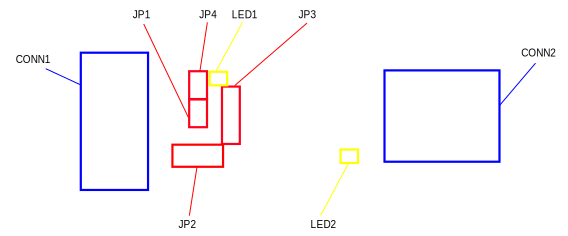
\includegraphics{images/usbprog_components}
  \caption{The USBprog device (version 3.0) with all connectors, jumpers and LEDs}
  \label{fig:usbprog}
\end{figure}

\subsection{Connectors}
\label{sec:connectors}

\begin{description}
  \item[CONN1] is the output interface which is used to do something useful with the USBprog beside
    from blinking LEDs. For example if you use the \emph{avrispmk2} firmware, this is an ISP
    interface which is used to program microcontrollers.

  \item[CONN2] is obviously the USB connector which is used to connect your USBprog to the computer.
    You have to use a \emph{Type B} cable which is the normal cable to connect USB devices---apart
    from micro or mini USB.
\end{description}


\subsection{Jumpers}
\label{sec:jumpers}

\begin{description}
  \item[JP1] (the lower two of the four pins) is the jumper that must be connected if the bootloader
    of the USBprog should be updated. See also section \vref{sec:inithardware} how to flash the
    bootloader.

  \item[JP2] controls how the power supply of the circuit that should be programmed (connected to
    \texttt{CONN1}). Figure \vref{fig:jp2} shows the possible connections:

    The default is no power supply for the programmed circuit. In that case you must ensure that the
    device is supplied with power by other means. This is the safest possibility.

    If you connect the two leftmost pins, that means that the 5~V VCC is directly from the USB port.
    This setting is dangerous because an error (short-circuit) in your circuit can damage the
    computer.

    An alternative is the setting of the two leftmost pins: In that case, the 5~V VCC is not
    directly from the USB port but with a Schottky diode. This is safer than the direct connection.

  \item[JP3] has two functions: At first it can be used as 5~V serial interface for debugging. You
    cannot directly connect this jumper to the computer but you need some level converter in
    between\footnote{If you want to build such a level converter yourself, look for example at
    \url{http://www.nslu2-linux.org/wiki/HowTo/AddASerialPort}. If you want to buy such a cable in
    Germany, the \href{http://www.eproo.net}{Embedded Project Shop} also has one. Look for
    ``FTDI-Kabel TTL-232R USB zu TTL serielles Kabel (5.0 V)''.}. This functionality is only needed
    by firmware developers.

    More important is another function which is used by the bootloader at startup. To put the device
    in update mode, disconnect the device, then connect pins 2 and 3 as shown in figure
    \vref{fig:jp3} and connect the device again.

  \item[JP4] is application specific, i.\,e. used directly by the firmware that is flashed into the
    USBprog. Currently, \texttt{JP4} is not used by any of the public firmwares.
\end{description}

\begin{figure}[thb]
  \centering
  
\includegraphics{images/jp2}
  \caption{Possible connections of \texttt{JP2}}
  \label{fig:jp2}
\end{figure}

\begin{figure}[thb]
  \centering
  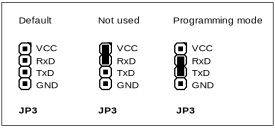
\includegraphics{images/jp3}
  \caption{Possible connections of \texttt{JP3}}
  \label{fig:jp3}
\end{figure}


\subsection{LEDs}
\label{sec:leds}

\begin{description}
  \item[LED1 (red)] is used by the firmware. There are two common scenarios:

    If the USBprog is in \emph{update mode,} the LED blinks slowly. In the wide-spread Atmel MTK II
    clone firmware, this LED shines while the programming of the microcontroller is ongoing.

  \item[LED2 (green)] is just the Power LED.
\end{description}


\section{Initialise the Hardware}
\label{sec:inithardware}

This section describes how to install the bootloader. If you bought a version of USBprog which
already contains the bootloader, you can safely skip that step. If you don't know if you have a
version with bootloader, please read section \vref{sec:check_if_bootloader_installed}.


\subsection{Check if the Bootloader is Installed}
\label{sec:check_if_bootloader_installed}

To check if the device already contains a bootloader, just put the device into programming mode
manually. For this step, you don't require any specific PC software. You just need a working USB
port.

\begin{enumerate}
  \item Disconnect your USBprog from the computer if it's connected.
  \item Close the jumper \texttt{JP1} as described in section \vref{sec:jumpers}.
  \item Connect the USBprog to a USB port.
\end{enumerate}

If \texttt{LED1} (see figure \vref{fig:usbprog}) now blinks, everything is fine. If not, there's no
working bootloader and you need to flash it.


\subsection{Flashing the Bootloader}

When buying a USBprog at the \href{http://www.eproo.net}{Embedded Projects Webshop} you can choose
between a slightly cheaper version without an already flashed bootloader and a slightly more
expensive version that already has flashed the bootloader.

Flashing the bootloader is the only step where you need a second programming device. It's possible
to use an already initialised USBprog with the ``AVRISP mk2 Clone'' firmware flashed. Any other
programmer for Atmel AVR microcontrollers will do it, too. You need the standardised \emph{ISP}
interface.

We need not only a programmer but also a programming software. While there are plenty of programmers
for Atmel AVR microcontrollers, we use \href{http://www.nongnu.org/avrdude/}{AVRdude} because it
supports quite a lot of hardware devices and it's available on basically any platform that is around
there. On Windows, we suggest to use \href{http://winavr.sourceforge.net/}{WinAVR} which is quite
easy to install.

\subsubsection{Setting the Jumpers}

To program the microcontroller that is on the USBprog board, you have to connect jumper
\texttt{JP1} as described in section \vref{sec:jumpers}.

There are two possibilities how the programmer gets its power:

\begin{enumerate}
  \item The programmer has its own power supply. That is the case for every USB-based programmer
    since USB can supply the device with up to 500~mA.
  \item The programmer takes the power from the circuit that should be programmed. That is the case
    for most ``self-made'' parallel port programmers since the parallel port is not able to supply
    devices with power.
\end{enumerate}

If you have a device of the second category, you have to set the jumper \texttt{JP2} as described in
section \vref{sec:jumpers} and shown in figure \vref{fig:jp3}. We suggest the 3rd method with the
Schottky diode.

\subsubsection{Wiring}

After the jumpers are right, connect the USBprog with a free USB port of your computer which is
necessary to supply the USBprog with power. The green power LED (\texttt{LED1}, see section
\vref{sec:leds}) indicates that everything is okay. If necessary connect your programmer with power
and with your computer.

For the connection between your programmer and your computer you need a 10-pole ribbon cable. The
pin assignment is the standardised ISP interface as shown in table \vref{tab:isp}. The numbering
scheme is shown in figure \vref{fig:isp}.

\begin{table}[ht]
  \centering
  \begin{tabular}{|p{1cm}p{5cm}|p{1cm}p{5cm}|}
    \hline
    \textbf{Pin} & \textbf{Description} & \textbf{Pin} & \textbf{Description} \\
    \hline
    \hline
    1            & MOSI (data out)       & 2            & VCC (+5~V)           \\
    3            & --                    & 4            & GND (signal ground)  \\
    5            & RESET                 & 6            & \verb+"+             \\
    7            & SCK (clock)           & 8            & \verb+"+             \\
    9            & MISO (instruction in) & 10           & \verb+"+             \\
    \hline
  \end{tabular}
  \caption{ISP Pin Assignment}
  \label{tab:isp}
\end{table}

\begin{figure}[tb]
  \centering
  
\includegraphics{images/isp}
  \caption{Pin numbering used in the ISP pin assignment}
  \label{fig:isp}
\end{figure}

\subsubsection{Flashing the Firmware}

Now it's time to flash the firmware with AVRdude. At first you have to find out how your programmer
is named in AVRdude which is listed in \cite{AVRdude} where the \texttt{-c} option is described.
This symbolic name is spelled as \texttt{PROGRAMMER} in the commands below.

At first you have to download the firmware file at
\url{http://svn.berlios.de/svnroot/repos/usbprog/trunk/usbprog\_base/firmware/usbprog\_base.hex}.
Save the file as \texttt{usbprog\_base.hex}.

Now flash the firmware with the command

\begin{lstlisting}[style=inline]
% avrdude -p m32 -c PROGRAMMER -U flash:w:usbprog_base.hex
\end{lstlisting}

The second step requires to set the fuse bits with following interactive AVRdude session:

\begin{lstlisting}[style=inline]
% avrdude -p m32 -c PROGRAMMER -t
avrdude> write lfuse 0 0xe0
avrdude> write hfuse 0 0xd8
avrdude> quit
\end{lstlisting}

After everything was successful, disconnect the USBprog, remove the jumper \texttt{JP1} and connect
the USBprog again. The red LED blinks now. This is a sign that you're ready to upload a firmware
which is described in section \vref{sec:firstfirmware}---just the next section!


\chapter{Getting Started with the Software}

\section{Installation}
\label{sec:installation}

\subsection{Binary Packages for Linux}
\label{sec:linux_binary_installation}

This section describes the installation of binary packages on wide-spread Linux distributions. If
you have a more exotic Linux distribution, another Unix flavour or if you just want to use the
latest and greatest version, proceed by reading section \vref{sec:compilingfromsource}.

In any case: After the installation has finished, the program can be started using \texttt{usbprog}
in a shell for the command line version of the USBprog software and \texttt{usbprog-gui} for the
graphical user interface (if installed). In the last case, USBprog should also appear in the start
menu of your desktop environment\footnote{At least if you use KDE, GNOME or Xfce.}, at least after
logging out and logging in again.

\subsubsection{Ubuntu/Debian}

That's the easiest distribution because Uwe Herrman (\url{uwe@debian.org}) was so kind to provide
Debian packages. Because everything that is in Debian is also in \emph{Universe,} you also have that
advantage on Ubuntu.

So: Just open a Terminal and install USBprog by entering

\begin{lstlisting}[style=inline]
% sudo aptitude install usbprog
\end{lstlisting}

If you also want to use the graphical interface of the USBprog software, use

\begin{lstlisting}[style=inline]
% sudo aptitude install usbprog usbprog-gui
\end{lstlisting}

The only ``disadvantage'' of installing the GUI is that it probably will install some dependencies
like wxGtk.

If you want to access the USBprog as user, that user has to be put in the \texttt{plugdev} group. To
do so, just execute (replace \texttt{@@USERNAME@@} with the username that you want to put into that
group):

\begin{lstlisting}[style=inline]
% sudo usermod -aG plugdev @@USERNAME@@
\end{lstlisting}

\subsubsection{openSUSE and SLES}

There are binary packages in the \href{https://build.opensuse.org/}{openSUSE Build Service},
directly from the author. So they should be always up to date. They are in the \emph{electronics}
repository. To add the repository to your package list, open a shell and then enter

\begin{lstlisting}[style=inline]
% sudo zypper ar -r http://repos.opensuse.org/electronics/@@DIST@@/electronics.repo
\end{lstlisting}

The term \texttt{@@DIST@@} has to be substituted version of your openSUSE or SLES as shown in table
\vref{tab:susedistributions}.

\begin{table}[ht]
  \centering
  \begin{tabular}{|p{4cm}p{10cm}|}
    \hline
    \textbf{String}                 & \textbf{Distribution}                               \\
    \hline
    \hline
    \texttt{openSUSE\_11.0}         & openSUSE 11.0                                       \\
    \texttt{openSUSE\_11.1}         & openSUSE 11.1                                       \\
    \texttt{openSUSE\_11.2}         & openSUSE 11.2                                       \\
    \texttt{SUSE\_Linux\_Factory}   & openSUSE Factory (the unstable development version) \\
    \texttt{SLE\_10}                & SUSE Linux Enterprise (Desktop/Server) 10           \\
    \texttt{SLE\_11}                & SUSE Linux Enterprise (Desktop/Server) 11           \\
    \hline
  \end{tabular}
  \caption{SUSE Distribution strings for the \emph{electronics} Build Service repository}
  \label{tab:susedistributions}
\end{table}

After that, refresh the package list with

\begin{lstlisting}[style=inline]
% sudo zypper ref
\end{lstlisting}

You're now ready to install USBprog:

\begin{lstlisting}[style=inline]
% sudo zypper install usbprog usbprog-gui
\end{lstlisting}

If you don't need the graphical user interface, just omit the \texttt{usbprog-gui} package. Of
course, since the repository is now known by the package manager, you can also install or uninstall
the USBprog packages using YaST.

If you want to access the USBprog as user, that user has to be put in the \texttt{uucp} group. Just
use YaST to perform that task. See also \texttt{/usr/share/doc/packages/usbprog/README.SUSE}.

\subsubsection{Fedora, CentOS and RHEL}

You may be surprised, but the binary packages for Fedora, Red Hat and CentOS are also built in the
\href{https://build.opensuse.org/}{openSUSE Build Service}. The only difference of that section
compared with the previous section is that we describe \texttt{yum} instead of \texttt{zypper} here.

There's no command so add a repository in \texttt{yum}. Instead, you have to change to the directory
\texttt{/etc/yum.repos.d} and download the repository file. In that case, you have to substitute
\texttt{@@DIST@@} with values of table \vref{tab:redhatdistributions}.

\begin{lstlisting}[style=inline]
% su
# cd /etc/yum.repos.d
# wget http://repos.opensuse.org/electronics/@@DIST@@/electronics.repo
\end{lstlisting}

\begin{table}[htb]
  \centering
  \begin{tabular}{|p{4cm}p{10cm}|}
    \hline
    \textbf{String}                 & \textbf{Distribution}                               \\
    \hline
    \hline
    \texttt{Fedora\_11}             & Fedora 11                                           \\
    \texttt{Fedora\_12}             & Fedora 12                                           \\
    \texttt{CentOS\_5}              & CentOS 5                                            \\
    \texttt{RHEL\_5}                & Red Hat Enterprise Linux 5                          \\
    \hline
  \end{tabular}
  \caption{Distribution strings for Red Hat-like distributions in the Build Service}
  \label{tab:redhatdistributions}
\end{table}

Since the refresh is done automatically by \texttt{yum}, just install the package(s) with

\begin{lstlisting}[style=inline]
# yum install usbprog usbprog-gui
\end{lstlisting}

As with SUSE and Ubuntu, you can omit the \texttt{usbprog-gui} package if you don't plan to use the
graphical user interface.

If you want to access the USBprog as user, that user has to be put in the \texttt{uucp} group on
RHEL/CentOS 5 or in the \texttt{dialout} group on recent Fedora versions. Just execute

\begin{lstlisting}[style=inline]
% sudo usermod -aG uucp @@USERNAME@@     # RHEL 5, CentOS 5
% sudo usermod -aG dialout @@USERNAME@@  # Fedora > 10
\end{lstlisting}

where \texttt{@@USERNAME@@} has to be replaced with the login of the user that should be in that
group.  See also \texttt{/usr/share/doc/usbprog/README.\{CentOS,Fedora,RedHat\}}.

\subsection{Windows}

\subsubsection{Supported Systems}

This section describes the installation of USBprog on Windows. Although binary packages are
provided, the installation is not trivial since we need to install a device driver---unlikely the
other operating systems that are able to handle USB devices in userspace without driver
installation.

At first, make sure that you're running one of following operating systems:

\begin{itemize}
  \item Windows 2000 with SP4
  \item Windows XP with SP3 (32 bit only)
  \item Windows Vista with SP1 (32 bit or 64 bit)\footnote{I was not able to test Windows Vista since
    I don't have it. The problem that prevented other USB devices from working after the
    installation of the USBprog software should be resolved at Windows 7 also was affected and
    Windows 7 works now.}
  \item Windows 7 (32 bit or 64 bit)
\end{itemize}

Although the installation package is prepared to run on a 64 bit Windows, I was not able to test it.
If you are successfully able to use it, please drop me a \href{bernhard@bwalle.de}{note}.

\subsubsection{Getting the Software}

\textbf{Note:} Please install the software \emph{before} attaching the hardware the first time. That
makes it easier for you. If you already attached the hardware, abort the driver installation
process.

You can download the latest Windows installer package at following site:

\ding{224} \url{http://developer.berlios.de/project/showfiles.php?group_id=7642}

There's only one installer package for both 32 and 64 bit Windows. While the userspace program is
always 32 bit, the driver is available as 32 bit and 64 bit version. Windows (like Linux) can handle
32 bit software on x86-64\footnote{also known as ``x64'' or ``amd64''}, but drivers have to be 64
bit.


\subsubsection{Installation of the Software}

Installation of the \emph{userspace software} (that excludes the driver part) is as easy as
installing any other Windows program. Just start the installer with a double click, confirm the
license, confirm the installation path and you're done.

To start the graphical user interface, select ``Start'' $\rightarrow$ ``USBprog''
$\rightarrow$ ``USBprog GUI''. The command line interface has the name ``USBprog Commandline''.

To uninstall the software, just use the ``Uninstall'' entry in the start menu or go to ``Control
Panel'' $\rightarrow$ ``Software''.


\subsubsection{Driver Installation on Windows 2000 and XP}

After you downloaded the software, the driver is located at \texttt{c:\textbackslash{}Program
Files\textbackslash{}USBprog\textbackslash{}driver} on an English Windows. Replace the ``Program
Files'' with something locale-specific like ``Programme'' in a German Windows installation.

To install the driver, perform these steps. We assume that you successfully installed the bootloader
on the device as described in section \vref{sec:inithardware}.

\begin{enumerate}
  \item Insert jumper \texttt{JP1} (see section \vref{sec:jumpers}) to put the device into
    programming mode after power up.
  \item Connect the device.
  \item After a few seconds, the ``New Hardware Wizard'' should appear.
  \item Don't connect with \emph{Windows Update}---you don't find a driver for the USBprog there.
  \item Choose ``Install from a list or specific location (Advanced)''.
  \item Select ``Search for the best driver in these locations'' and tick ``Include this location in
    the search''.
  \item Choose ``Browse'' and select the driver directory mentioned above \newline
    (\texttt{c:\textbackslash{}Program Files\textbackslash{}USBprog\textbackslash{}driver}).
\end{enumerate}

That's it. Figure \vref{fig:inst_winxp} shows screenshots of the dialogs (German only). To test your
installation, fire up the USBprog software. In the command line mode, \texttt{devices} should list
exactly one USBprog device and in GUI mode, the combo box should have also an entry.

\begin{figure}[p]
  \centering
  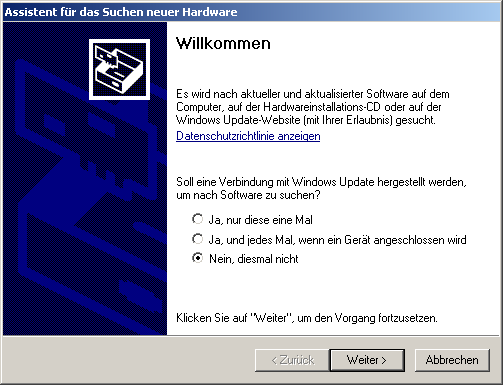
\includegraphics[width=92mm]{images/win_xp_1.png}
  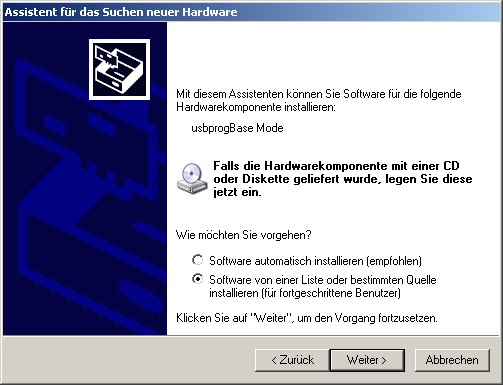
\includegraphics[width=92mm]{images/win_xp_2.png}
  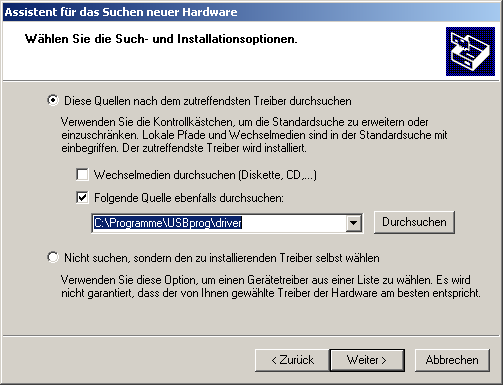
\includegraphics[width=92mm]{images/win_xp_3.png}
  \caption{Installation workflow on Windows XP (German only)}
  \label{fig:inst_winxp}
\end{figure}

\subsubsection{Driver Installation on Windows Vista and 7}

The following procedure describes only Windows 7, but Windows Vista should be similar.  To install
the driver, perform these steps. We assume that you successfully installed the bootloader on the
device as described in section \vref{sec:inithardware}.

\textbf{Note:} If you have a 64 bit version of Windows Vista or 7, you cannot install unsigned
device drivers by default. However, there's a software called
\href{http://www.ngohq.com/home.php?page=dseo}{Driver Signature Enforcement
Overrider} that should solve that problem. Use the software at own risk---sorry!

Okay, let's start: At first you need to insert jumper \texttt{JP1} (see section \vref{sec:jumpers})
to put the device into programming mode after power up. Then connect the device. Now Windows looks
for a matching driver and doesn't find one. This procedure takes about one minute\footnote{at least
in my installation in VirtualBox, maybe a native Windows is much faster} and then the dialog shown
in figure \vref{fig:windows_no_driver} appears.

\begin{figure}[ht]
  \centering
  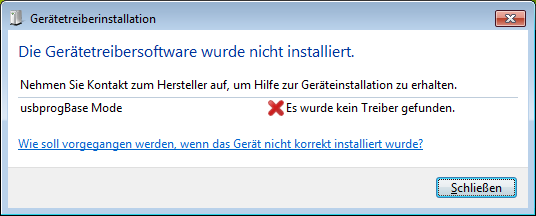
\includegraphics[scale=.7]{images/win7_1.png}
  \caption{No driver has been found (German only)}
  \label{fig:windows_no_driver}
\end{figure}

So we have to install the driver manually:

\begin{enumerate}
  \item Open the ``Device Manager''. You find it in ``Control Panel'' $\rightarrow$ ``Hardware and
    Sound'' $\rightarrow$ ``Devices and Printers'' $\rightarrow$ ``Device Manager''.

  \item The device ``usbprogBase Mode'' should appear there with a little warning sign as shown in
    figure \vref{fig:windows_manual_driver} in the first picture. Select ``Update driver''. 

  \item Windows asks you where you want to search for the driver (figure
    \vref{fig:windows_manual_driver}, second picture). Choose to manually specify the location
    and select \texttt{c:\textbackslash{}Program Files\textbackslash{}USBprog\textbackslash{}driver}
    then.

  \item A red warning that the driver is not signed appears (figure
    \vref{fig:windows_manual_driver}, third picture). Confirm the driver installation!
\end{enumerate}

\begin{figure}[p]
  \centering
  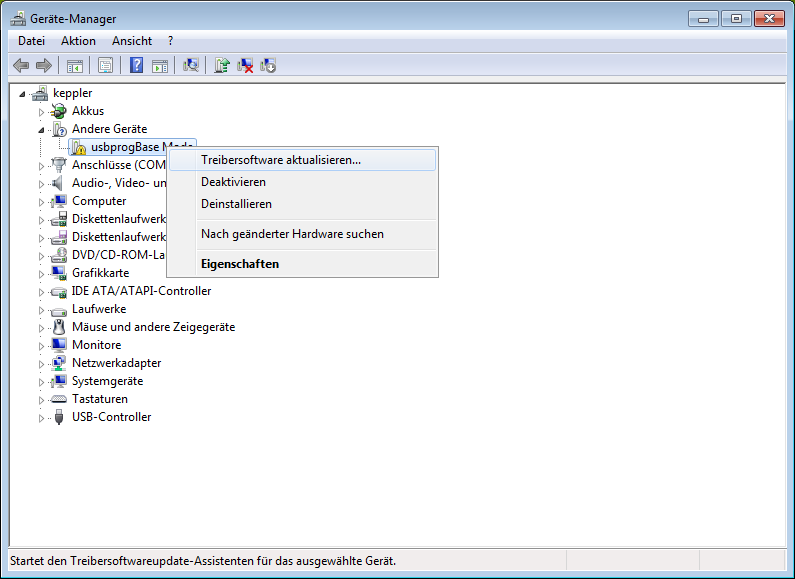
\includegraphics[scale=.58]{images/win7_2.png} \\[1mm]
  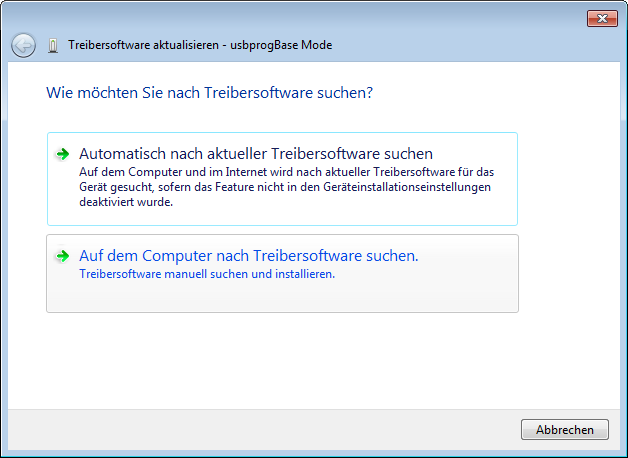
\includegraphics[scale=.58]{images/win7_3.png} \\[1mm]
  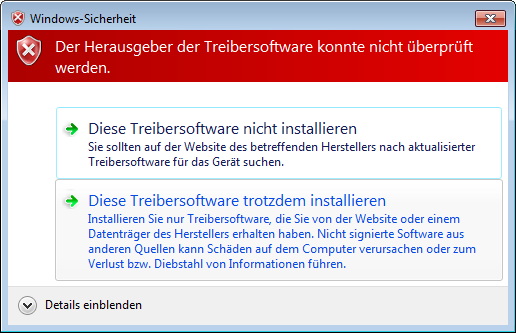
\includegraphics[scale=.58]{images/win7_4.png}
  \caption{Manual driver installation on Windows (German only)}
  \label{fig:windows_manual_driver}
\end{figure}

That's it. To test your installation, fire up the USBprog software. In the command line mode,
devices should list exactly one USBprog device and in GUI mode, the combo box should have also an
entry.

\subsection{MacOS}

Porting Unix software to the Mac is easy, but developing cross-platform software that feels really
MacOS-like is hard---especially if you are software developer and not designer.  Therefore, we don't
provide a software package for the Mac. But nevertheless: It's easy to install the USBprog software
on the Mac.

You can compile USBprog directly from the source as described in section
\vref{sec:compilingfromsource}. However, it's more easy if you use \emph{MacPorts}. Just install
MacPorts on your computer as described in \cite{InstallingMacports}.

After that, open a Terminal and execute

\begin{lstlisting}[style=inline]
% sudo port install usbprog
\end{lstlisting}

After that, you can start the command line tool with \texttt{usbprog} in a shell and the GUI with
\texttt{usbprog-gui}.


\subsection{Compiling USBprog from Source}
\label{sec:compilingfromsource}

\subsubsection{Operating Systems}

This section describes how to build USBprog from source. Sometimes there are valid reasons that even
``normal'' users (and not developers) wish to compile the program from the source code:

\begin{itemize}
  \item a newer version is available that fixes a bug but the distribution package is too old;
  \item a more ``exotic'' Linux distribution is used for which no binary packages are available;
  \item even another operating system (not Linux or MacOS) is used.
\end{itemize}

Therefore, that section describes how to compile USBprog on Unix (which includes MacOS).  Compiling
it on Windows is completely different. Since there is always a binary setup package is available on
that platform, the reasons mentioned above don't apply here. If you want to compile USBprog on
Windows, refer to the file \texttt{win32/README} in the USBprog source distribution.

\subsubsection{Dependencies}

When compiling software from source, care must be taken to ensure that all dependencies are
installed on the computer. The USBprog software needs following other software components. If you
use distribution packages to install these dependencies, ensure that the header files (usually in a
subpackage \texttt{-dev}\footnote{on Debian/Ubuntu} or \texttt{-devel}\footnote{on RPM-based
distributions like Red Hat or SUSE}) are installed, too.

\begin{itemize}
  \item a working C++ compiler like \texttt{g++};
  \item Perl (\url{http://www.perl.org}) to build the manual pages from the POD sources;
  \item libusb (\url{http://www.libusb.org});
  \item libxml (\url{http://www.xmlsoft.org});
  \item libcurl (\url{http://curl.haxx.se});
  \item GNU Readline (\url{http://tiswww.case.edu/php/chet/readline/rltop.html}) only if you want to
    use command-line completion with \texttt{TAB};
  \item wxWidgets (\url{http://www.wxwidgets.org}) only if you want to build a graphical user
    interface.
\end{itemize}

\subsubsection{Download, Build and Install}

After everything is fine, download the source tarball from following source:

\ding{224} \url{http://developer.berlios.de/project/showfiles.php?group_id=7642}

You should have a file called \texttt{usbprog-@@VERSION@@.tar.bz2} on the disk where
\texttt{@@VERSION@@} represents the version of the program. At first, extract that tarball and
change into the newly created directory afterwards:

\begin{lstlisting}[style=inline]
% tar xvfj usbprog-@@VERSION@@.tar.bz2
% cd usbprog-@@VERSION@@/
\end{lstlisting}

Now configure the software using

\begin{lstlisting}[style=inline]
% ./configure
\end{lstlisting}

Lots of text messages appear. If the last lines look like

\begin{lstlisting}[style=inline]
---------------------------------------------------
           Build summary
---------------------------------------------------
Readline         : enabled
GUI (wxWidgets)  : enabled
---------------------------------------------------
\end{lstlisting}

everything is fine. Of course ``disabled'' is also okay, but then the specific feature is missing!

Build and install the software with

\begin{lstlisting}[style=inline]
% make
% sudo make install # or su -c "make install"
\end{lstlisting}

You can now start the software with \texttt{usbprog} (the CLI variant) or \texttt{usbprog-gui} (the
graphical user interface, if built) and should also find it in the menu of your desktop environment.
Also, a manual page should be available, both \emph{usbprog(1)} and \emph{usbprog-gui(1)}.

\subsubsection{Hardware Access for Normal Users}

\textbf{Note:} This applies only to Linux. For other operating systems please refer to the
documentation of the system vendor or simply stick to \texttt{root}.

By default, only the \texttt{root} user has ``raw'' access to USB devices. Since it's not desirable
to start USBprog---especially the graphical user interface---always as \texttt{root}, we have to
change system configuration in a way that it allows non-root users the access to the device.

Whenever a new device is detected on the system, the kernel asks a superspace deamon called
\emph{udev} to create a new device node below \texttt{/dev}. For USB devices, the raw device file
(that gets accessed by \emph{libusb} applications like USBprog) is below \texttt{/dev/bus/usb}. The
permission of that device file determines which user has access to that device file.

A simple solution is now to create a \emph{udev rule} that gives that device file not
\texttt{root:root} but \texttt{root:@@GROUP@@} with write permission for that group. All users that
should be allowed to use USBprog can not be put in \texttt{@@GROUP@@}.

A template for that udev rule is distributed with the USBprog source distribution called
\texttt{usbprog.rules.in}.  Replace the term \texttt{@@USBPROG\_GROUP@@} with the name of the group
you want to use\footnote{You can create a new group called \texttt{usbprog} or you can simple re-use
an existing group like \texttt{plugdev} on Ubuntu for storage devices.} and copy the file in
\texttt{/etc/udev/rules.d}.  Since the lexicographic order in that directory determines the priority
(processing order) of rules, it's quite common to prefix it with a number. Example:

\begin{lstlisting}[style=inline]
% sed -e 's/@@USBPROG_GROUP@@/plugdev/g' usbprog.rules.in \
  > /etc/udev/rules.d/98-usbprog.rules
\end{lstlisting}

Of course ``modern'' Linux distributions (especially Red Hat and SUSE flavours) offer more
complicate solutions to give the current ``desktop'' user more permission to the devices. However,
that solutions are not standardised, tend do change every year and sometimes even are poorly
documented. Therefore, we don't describe that here. For the average user, this group-based solution
is sufficient.

However: You don't want to use that solution in a centrally administered company network. Contact
your system administrator instead. \texttt{:-)}

\section{The Update Mode}

\subsection{How USB Works}

\subsubsection{USB Device Identification}

You don't know much about USB to use USBprog. However, one fact is important to understand the
limitations of the USBprog especially on Microsoft Windows: How a USB device is identified.

Whenever you connect a USB device to the computer, the USB \emph{host} (the computer) asks the USB
\emph{device} a few things. This process is called \emph{enumeration}. After the enumeration process
has finished, the USB host assigns the USB device an address. On Linux, this process can be watched
in the kernel log with the \texttt{dmesg} command:

\begin{lstlisting}[style=inline]
usb 6-1: new full speed USB device using uhci_hcd and address 2
usb 6-1: New USB device found, idVendor=1781, idProduct=0c62
usb 6-1: New USB device strings: Mfr=1, Product=2, SerialNumber=0
usb 6-1: Product: usbprogBase Mode
usb 6-1: Manufacturer: USBprog EmbeddedProjects
usb 6-1: configuration #1 chosen from 1 choice
\end{lstlisting}

As already mentioned in section \vref{sec:definitions}, the USBprog device has a special
\emph{bootloader} that allows the \emph{firmware} to be updated without another device.
When you connect the USBprog to the computer, the device normally starts the firmware.
If you have flashed for example the \texttt{avrispmk2} firmware, then the device identifies as
``Atmel AVR ISP mkII''\footnote{USB Vendor ID: 0x03eb, USB Device ID: 0x03eb}.

\textbf{Important:} Although the USBprog is always the same hardware device, depending on the
operation mode and the firmware, it is seen as totally different devices from the computer's point
of view. It can even change its identity at runtime without re-attaching!

\subsubsection{USB Drivers on Windows}

Two important things have to be considered when using USB Devices on Microsoft Windows:

\begin{itemize}
  \item It \emph{does} matter on which USB port a device is connected for a driver. So if you
    connect the device to a different USB port, the driver installation process has to be repeated.
    However, since Windows knows the driver from the last time, everything goes
    automatically---which doesn't Windows prevent from displaying lots of dialogues.

  \item You need a device driver\footnote{One exception are HID drivers which can be accessed from a
    userspace application.} for each device.
\end{itemize}

While the first fact is only a bit annoying, the second fact matters when using the USBprog: Since
the device can change its identity at runtime, after the identity changes, a new device driver has
to be installed. And it's not possible to access the USBprog device while it emulates another device
like the Atmel AVR ISP mkII.

However: In normal operation, that's not a problem. I just wanted to explain that fact so that you
understand why the manual switch to the update mode is necessary.

\bibliographystyle{IEEEtran}

\subsection{Switching to the Update Mode}
\label{sec:switch_updatemode}

Whenever the firmware (not the bootloader) of the USBprog needs to be updated, the device must be
switched from normal operation mode to update mode. There are two ways of putting the USBprog in
update mode:

\begin{enumerate}
  \item Sending some magic stuff to the device that puts the USBprog in update mode at normal
    operation runtime.
  \item Disconnecting the device, setting jumper \texttt{JP1} (see section \vref{sec:jumpers})
    and connecting the device again.
\end{enumerate}

While the first variant seems to be easier (especially when developing a new firmware where you have
to re-flash the USBprog every few minutes), it clearly has its disadvantages: It doesn't work on
Windows for the reasons already explained and it sometimes doesn't seem to work reliably at all.

Therefore: As ordinary user, we always recommend to use the jumper to switch to update mode! After
programming, the USBprog automatically switches from update mode to normal mode\footnote{yes, even
on Windows}. So don't forget to remove the jumper to prevent the USBprog from starting in update
mode at next time you connect the USBprog again or the computer boots.

To detect if the firmware is in update mode---you may already have noticed it---the red LED flashes
in a sequence ``flash, flash, pause, flash, flash, \ldots''.


\section{Upload the First Firmware}
\label{sec:firstfirmware}

We describe the command line interface here as ``first step'' for a simple reason: It's exactly the
same on every platforms and a command can be reproduced by the user more easily than finding GUI
elements.

So open a shell on Unix (Linux/MacOS) or open the ``USBprog Commandline'' in the ``Start'' menu on
Windows. You should see a prompt that looks like

\begin{lstlisting}[style=inline]
(usbprog) _
\end{lstlisting}

Now connect the USBprog device with the \texttt{JP1} (update mode) jumper set.  After you connected
the USBprog to the USB port of your computer, wait a few seconds to make sure that the operating
system detected the device.

Back to the USBprog software, the \texttt{devices} command should display a single USBprog device:

\begin{lstlisting}[style=inline]
(usbprog) devices
 [ 0]  *  Bus 003 Device 002: 1781:c620
          usbprog: USBprog in update mode
\end{lstlisting}

Since it's the only device and since the device is already in \emph{update mode,} the star
(\texttt{*}) after the number shows you that this device is already selected. So you can proceed and
upload the \texttt{blinkdemo} firmware. That firmware does nothing but blinking the LED. Blinking
the LED you ask? It's already blinking! Well, the sequence is different, so it should be easily
possible to distinguish the \texttt{blinkdemo} blinking from the update mode blinking.

Enough talking. Let's now upload the firmware:

\begin{lstlisting}[style=inline]
(usbprog) upload blinkdemo
Opening device ...
Writing firmware ...
###############################################################################
Starting device ...
Detecting new USB devices ...
\end{lstlisting}

Okay, that's it! The next chapters describe both the GUI and the command line in detail. If you then
want to do something real with your USBprog like programming an AVR microcontroller, read chapter
\vref{sec:commonfirmwares}.

\chapter{USBprog Software Reference}

\section{The Firmware Pool}

\subsection{Overview}
\label{sec:firmwarepool_overview}

Both the GUI and the command line use the firmware pool available in the internet. Therefore, you
need an internet connection to use USBprog, at least at the first time. Since the firmware pool is
cached on the disk, you can also use USBprog without an internet connection later.

To get the list of available firmware files, USBprog will connect to the internet at startup and
download the file \url{http://www.ixbat.de/usbprog/versions.xml}. So if you run some ``personal
firewall'' software on Windows and that software asks you if it's okay to connect to the internet,
that's because of that file.

Right of the label ``Online Pool'', there's a combo box with all the firmwares available at the
firmware pool. Before uploading a firmware to the USBprog device, you probably want to get some
information for the firmware first.

\subsection{Location of the Cache}

For the curious, here's the location of the firmware cache where also the \texttt{version.xml} file
is downloaded:

\begin{itemize}
  \item \textbf{Linux/MacOS:} \texttt{\$HOME/.usbprog}
  \item \textbf{Windows:} \texttt{\%APPDATA\%} (just enter that in the Explorer and it shows you
    the directory in your Windows installation), for example: \\
    \texttt{c:\textbackslash{}Documents and Settings\textbackslash{}bwalle\textbackslash{}Anwendungsdaten}
\end{itemize}

\section{Configuring a Proxy}

The USBprog software uses \emph{libcurl} for internet access. Therefore, it honours the environment
variable \texttt{http\_proxy} that simply can be set to the hostname of the proxy. Read the manpage
\emph{curl(1)} and the ``ENVIRONMENT'' section in specific for more information.

In addition to that settings, the Windows version of USBprog also honours the Internet Explorer proxy
settings. However, also on Windows, the environment variables overwrite the Internet Explorer
settings. If you are in doubt, set the environment since that's better documented and supported
directly by \emph{libcurl}.



\section{Graphical User Interface}
\label{sec:gui}

The installation instructions in section \vref{sec:installation} explain also how to start the
USBprog GUI. After the program has started, a window like figure \vref{fig:screenshot} should
appear. Of course the GUI looks different on the different operating system, but since the program
is built from the same sources using the cross-platform toolkit \emph{wxWidgets} the differences
should be small.

\begin{figure}[bp]
  \centering
  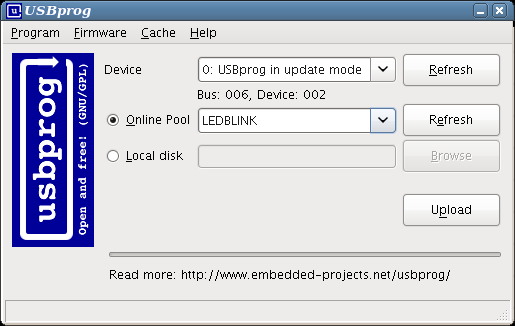
\includegraphics[scale=0.5]{images/usbprog_gui.png}
  \caption{Screenshot of USBprog on Linux}
  \label{fig:screenshot}
\end{figure}



\subsection{Getting Information for a Firmware}

Some very common firmwares are described in chapter \vref{sec:commonfirmwares} in that
documentation. However, for any firmware available, you can display some brief information.
Just select the firmware in the combo box and choose ``Firmware'' $\rightarrow$ ``Info'' or press
\texttt{F2}. A dialog like figure \vref{fig:screenshot_info} appears.

\begin{figure}[hp]
  \centering
  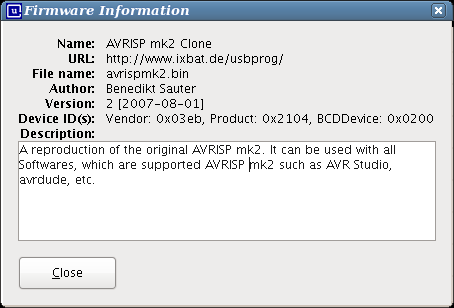
\includegraphics[scale=0.5]{images/usbprog_info.png}
  \caption{Information about the \texttt{avrispmk2} firmware}
  \label{fig:screenshot_info}
\end{figure}

If you want to get the pin assignment, choose  ``Firmware'' $\rightarrow$ ``Pins''  or press
\texttt{F3}. A dialog like figure \vref{fig:screenshot_info} appears.


\begin{figure}[hp]
  \centering
  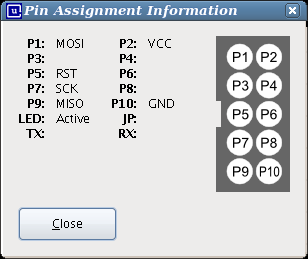
\includegraphics[scale=0.5]{images/usbprog_pin.png}
  \caption{Pin assignment of the \texttt{avrispmk2} firmware}
  \label{fig:screenshot_pin}
\end{figure}

\subsection{Cache Management Functions}

If you want to have all firmware files available for offline usage, just choose ``Cache''
$\rightarrow$ ``Download all''.

For cleanup, there are two different entries:

\begin{itemize}
  \item The ``Clean'' function only deletes unused firmware files that are still in the cache but
    are useless: Files that are not referenced in the index file (\texttt{versions.xml}) any more.
    This can be old versions of firmwares still in the index file or removed firmwares.

  \item The ``Delete cache'' function removes all firmware files from the cache.
\end{itemize}


\subsection{Uploading a Firmware}

Uploading a firmware from the online pool is easy:

\begin{enumerate}
  \item Connect the device in update mode (see section \vref{sec:switch_updatemode}).
  \item Select a device in the ``Device'' list. Maybe you need to click on ``Refresh'' first.
  \item Select a firmware in the ``Firmware'' list.
  \item Click on ``Upload''.
\end{enumerate}

The progress bar should tell you that there's a upload in process and the string ``Upload
successful'' should show up in the status bar. The software also starts the firmware immediately.
Don't forget to remove the \texttt{JP1} jumper!

If you want to upload a firmware that is not in the cache, click on the radio button ``Local disk''
and use ``Browse'' to select a full path to the firmware file (binary format). The rest is the same.

\subsection{Debugging}

If something doesn't work and you need support from the author (or any other party listed in section
\vref{sec:support}), a logfile is always helpful. To write a log file in the GUI, click on
``Program'' $\rightarrow$ ``Logging'' and select an appropriate path.

You can also start the application in logging mode:

\begin{lstlisting}[style=inline]
% usbprog-gui -D
\end{lstlisting}

This logs to standard error. To redirect that to a file, just use the redirection operator of the
shell (Unix only):

\begin{lstlisting}[style=inline]
% usbprog-gui -D 2> /path/to/logfile.log
\end{lstlisting}



\section{USBprog Command Line}
\label{sec:cli}

\subsection{Overview}

Why use the command line version if there's a GUI (section \vref{sec:gui})? There are several
reasons:

\begin{itemize}
  \item The command line version is available everywhere (for example on RHEL there's no
    \emph{wxWidgets} package, therefore it's much more work to get the GUI running).

  \item The command line version can be scripted.

  \item Some people like me prefer CLIs\footnote{Command Line Interface} over GUIs. \texttt{:-)}
\end{itemize}

Because the GUI and the command line use the same library, they should share all bugs and features.
They also share the cache.

The USBprog command line client works like a shell. Each command takes a fixed number of arguments.
If the argument is not specified, the shell asks for it:

\begin{lstlisting}[style=inline]
(usbprog) helpcmd
command> _
\end{lstlisting}

Also, some commands can be accessed via multiple names:

\begin{lstlisting}[style=inline]
(usbprog) helpcmd bla
Invalid command: bla
(usbprog) ? bla
Invalid command: bla
\end{lstlisting}

The best: If compiled with readline support which is the case for all binary packages listed in
section \vref{sec:linux_binary_installation}, \texttt{TAB} completion works like you would expect
it.


\subsection{Getting Help}

Because a CLI cannot be ``self-explanatory'', there are several ways to get a quick help beside from
that document. The command

\begin{lstlisting}[style=inline]
(usbprog) help
\end{lstlisting}

displays a list of all available commands. To get more help for a specific command, use
\texttt{helpcmd \emph{COMMAND}} or \texttt{? \emph{COMMAND}}. For example:

\begin{lstlisting}[style=inline]
(usbprog) ? pin
Name:            pin
Aliases:         pins
Argument:        firmware

Description:
Prints a list about pin usage. This might help you when connecting
something to your USBprog.
\end{lstlisting}

Last, but not least, the manual page \emph{usbprog(1)} briefly lists all commands and invocation
parameters.

\subsection{Exiting}

Well, it's quite obvious, but since the documentation should be complete, there are three ways to
exit the shell:

\begin{enumerate}
  \item The command \texttt{exit}.
  \item The alias \texttt{quit}.
  \item Sending a end-of-line (EOL) with \texttt{Ctrl-D} on Unix and \texttt{Ctrl-Z} on Windows.
\end{enumerate}

\subsection{Getting Information for a Firmware}

To view a list of firmware files in the pool (see section \vref{sec:firmwarepool_overview} for an
explanation of the firmware pool), use the command \texttt{list} like here:

\begin{lstlisting}[style=inline]
(usbprog) list
JTAGICE2      [ ] JTAGICE2
XSVF Player   [ ] XSVF Player
at89prog      [*] at89prog
avrispmk2     [*] AVRISP mk2 Clone
blinkdemo     [ ] LEDBLINK
openocd       [*] OpenOCD Debugger
simpleport    [*] SimplePort
usbprogrs232  [*] usbprogRS232

*: Firmware file downloaded
\end{lstlisting}

The star (\texttt{*}) shows if the firmware is already downloaded for offline usage. To display
information about a specific firmware, use \texttt{info \emph{FIRMWARE}} and \texttt{pins
\emph{FIRMWARE}}:

\begin{lstlisting}[style=inline]
(usbprog) info blinkdemo
Identifier   : blinkdemo
Name         : LEDBLINK
URL          : http://www.ixbat.de/usbprog/
File name    : blinkdemo.bin
Author       : Benedikt Sauter
Version      : 1 [2007-08-13]
Device ID(s) : Vendor: 0x1781, Product: 0x0c62, BCDDevice: 0x0001

Description
A simple LED blink demo.

For information about the Pin assignment, use the "pin blinkdemo" command.

(usbprog) pins blinkdemo
            +----------------+
            |  9  7  5  3  1 |
            | 10  8  6  4  2 |
            +----------------+

[   P1]               [   P2] 
[   P3]               [   P4] 
[   P5]               [   P6] 
[   P7]               [   P8] 
[   P9]               [  P10] 
[  LED] Blink LED     
\end{lstlisting}

\subsection{Uploading a Firmware}

Before you can upload a firmware, you must select a device first and---contrary to the GUI---you
must download the firmware file to the cache.

\subsubsection{Selecting a Device}

The \texttt{devices} command gives you a list of available updatable devices:

\begin{lstlisting}[style=inline]
(usbprog) devices
 [ 0]  *  Bus 006 Device 004: 1781:c620
          usbprog: USBprog in update mode
\end{lstlisting}

In that case, the device is already selected as update device. This is the case if there's only one
device available and if that device is already in update mode (see section
\vref{sec:switch_updatemode}). Otherwise, select the device with the \texttt{device \emph{NUMBER}}
command as update device:

\begin{lstlisting}[style=inline]
(usbprog) device 0
\end{lstlisting}

\subsubsection{Downloading the Firmware}

The \texttt{list} command shows you with the missing star (\texttt{*}) that the
\texttt{blinkdemo} is not downloaded. Just download the firmware with

\begin{lstlisting}[style=inline]
(usbprog) download blinkdemo
################################################################################
Firmware blinkdemo has been downloaded successfully.
\end{lstlisting}

\subsubsection{Uploading the Firmware}

It's recommended that you manually put the hardware in update mode as described in section
\vref{sec:switch_updatemode}. If that's not done and you selected another device as update device,
the software tries to put the device in update mode first\footnote{that does not work on Microsoft
Windows}.

In any case, just upload the firmware with \texttt{upload \emph{FIRMWARE}}:

\begin{lstlisting}[style=inline]
(usbprog) upload blinkdemo 
Opening device ...
Writing firmware ...
###############################################################################
Starting device ...
Detecting new USB devices ...
\end{lstlisting}

As the output indicates, the firmware starts immediately---in that case, the LED blink frequency
changes.

\subsubsection{Starting a Firmware}

If you now disconnect the device, leave the \texttt{JP1} jumper connected and connect the
device again, the device again shows in \emph{update mode}. However, we know that we flashed the
\texttt{blinkdemo} firmware. We could now remove the jumper and start it, or flash the firmware
again. But we could also use the \texttt{start} command:

\begin{lstlisting}[style=inline]
(usbprog) devices
 [ 0]  *  Bus 006 Device 006: 1781:c620
          usbprog: USBprog in update mode
(usbprog) start
Device successfully started.
\end{lstlisting}

The firmware starts, we see the blink frequency changing!





\subsection{Managing the Cache}

\subsubsection{Downloading Everything}

Of course it's also possible to download every firmware file with the command line interface. Just
use \texttt{download all}:

\begin{lstlisting}[style=inline]
(usbprog) download all
Downloading at89prog ...
################################################################################
Downloading AVRISP mk2 Clone ...
################################################################################
...
\end{lstlisting}

\subsubsection{Cleanup}

A cache cleanup can be done with the \texttt{cache \emph{OPERATION}} command. It has two functions:

\begin{itemize}
  \item If you just want to delete unused files, execute \texttt{cache clean}. That can be firmware
    files that are not referenced by the index file any more because they have been removed or the
    version has been increased.

  \item If you want to delete the full cache, use \texttt{cache delete}.
\end{itemize}

This example shows the effect of the last command:

\begin{lstlisting}[style=inline]
(usbprog) list
JTAGICE2      [ ] JTAGICE2
XSVF Player   [ ] XSVF Player
at89prog      [*] at89prog
avrispmk2     [*] AVRISP mk2 Clone
blinkdemo     [*] LEDBLINK
openocd       [*] OpenOCD Debugger
simpleport    [*] SimplePort
usbprogrs232  [*] usbprogRS232

(usbprog) cache delete 

(usbprog) list
JTAGICE2      [ ] JTAGICE2
XSVF Player   [ ] XSVF Player
at89prog      [ ] at89prog
avrispmk2     [ ] AVRISP mk2 Clone
blinkdemo     [ ] LEDBLINK
openocd       [ ] OpenOCD Debugger
simpleport    [ ] SimplePort
usbprogrs232  [ ] usbprogRS232
\end{lstlisting}

As you see, after the \texttt{cache delete} operation, no firmware is in the cache any more.


\chapter{Common Firmwares}
\label{sec:commonfirmwares}

\section{Atmel AVR ISP mkII Clone}

\begin{thebibliography}{99}
  \bibitem{AVRdude} AVRDUDE Manual,
    \url{http://www.nongnu.org/avrdude/user-manual/avrdude.html}

  \bibitem{InstallingMacports} ``Installing MacPorts'', \url{http://www.macports.org/install.php}
\end{thebibliography}

\end{document}

% vim: set sw=2 ts=2 et spell spelllang=en_gb tw=100:
